\chapter{Abstraction}

\section{Data Abstraction}
\begin{itemize}
    \item Data abstrction: a methodology by which functions enforce an abstraction barrier between \emph{representaion} and \emph{use}
    \item Identify a basic set of operations in which all manipulations of a data type can be expressed, then use only those operations for manipulating that data
    \item Abstraction barriers separate stages of an implementation into levels of abstraction
    \item Example - rational numbers:
    \medskip
	\begin{figure}[H]
	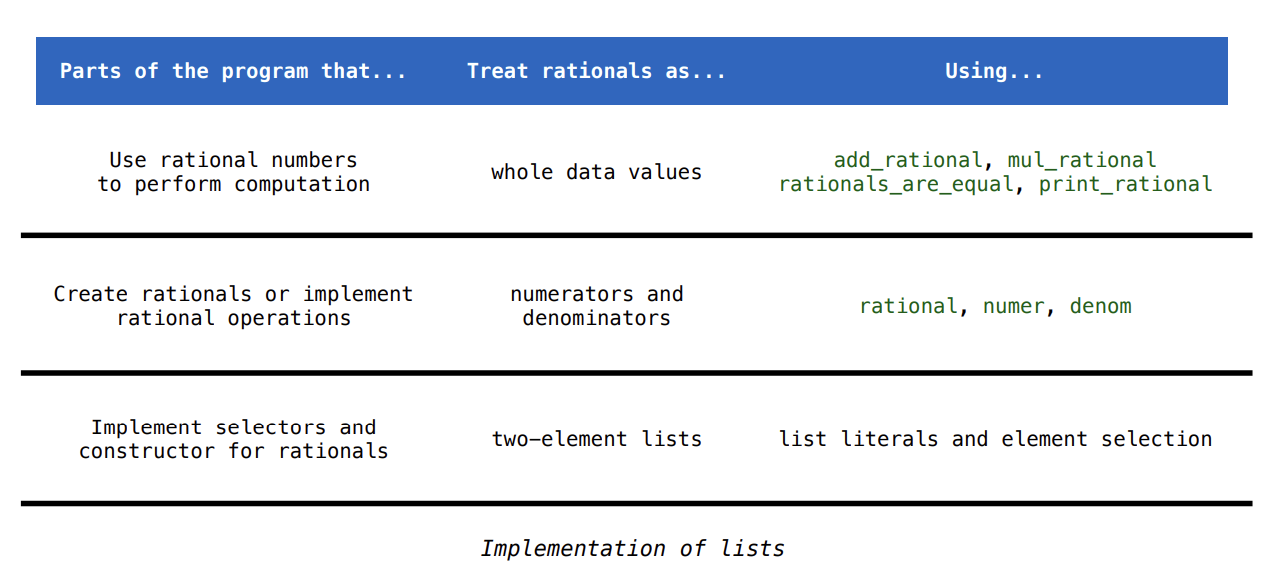
\includegraphics[width=1\linewidth]{figures/data_abstraction.png}
	\caption{List Format in Environment Diagrams}
	\end{figure}
\end{itemize}